\chapter{Développement expérimental}
\label{sec:chapxp}
\vspace*{-1cm}
Dans ce chapitre, nous détaillons le dispositif expérimental développé au cours de cette thèse. Le chapitre se divise en 4 sections, présentant le dispositif mécanique et les matériaux utilisés, puis les mesures électroniques et optiques implémentées sur le système.


\minitoc
\newpage

\section{Principe de l'expérience}
\label{sec:grossepresse}
\vspace{.5cm}

L'objectif du dispositif que nous avons développé est de permettre la compression et le cisaillement contrôlés de deux plaques minces de polyméthacrylate de méthyle (PMMA) de \qtyproduct[product-units=single]{150 x 80 x 10}{\mm} l'une sur l'autre. La compression s'effectue à position verticale imposée, et à force normale mesurée. Le cisaillement s'effectue à vitesse constante, et à force cisaillante mesurée. La force normale typique appliquée est de l'ordre de \SI{3000}{\N}, et le cisaillement est appliqué à une vitesse typique de \SI{20}{\micro\metre\per\second}. Le déplacement horizontal total imposé lors d'une expérience est typiquement de 6 à \SI{12}{\mm}, soit un temps d'expérience allant de 5 à 10 minutes.


\subsection{Presse mécanique}

Nous avons développé en partenariat avec Marc Moulin du Service d'Ingénierie Mécanique de l'ENS de Lyon une presse mécanique verticale contrôlée en position (Fig.\,\ref{fig:presse}).
Le déplacement vertical du bloc supérieur et l'application de la force normale se font par le biais d'une barre horizontale rigide équipée d'un capteur de force. Son déplacement, contrôlé en position par la rotation d'une vis, s'effectue par roulement sur des rails verticaux. Des patins rigides permettent un verrouillage de la position de la barre sur ces rails. Le déplacement tangentiel du bloc inférieur et l'application de la force cisaillante se font au moyen d'une platine de translation horizontale motorisée. Elle permet de translater le bloc inférieur tandis que le bloc supérieur reste fixe. Le bloc supérieur est
%disposé sur une platine de translation à roulement à billes 
solidaire d'un capteur de force, permettant la mesure de la force cisaillante exercée sur l'interface. Les échantillons pressés sont fixés au dispositif au moyen de mors métalliques dans lesquels ils sont encastrés d'un centimètre.

Du fait de la flexibilité des éléments mécaniques et de la géométrie du système, une faible rotation s'applique au bloc du haut lorsque le chargement cisaillant est appliqué. Pour compenser cette rotation, un système de vis permet d'assurer l'alignement des faces des deux blocs en contact, et d'homogénéiser les contraintes à l'interface.






\subsection{Mesure de force}

Deux capteurs de force sont installés sur la presse (Fig.\,\ref{fig:captforce}). La mesure de force par ces capteurs commerciaux repose sur une mesure des déformations engendrées par l'application d'une pression sur leurs faces par des jauges de déformation.
Les faces du capteur de force normale sont à cet effet solidaires respectivement de la vis de contrôle de la presse et de la barre horizontale, elle-même solidaire du bloc supérieur. Cette disposition permet à la vis d'appliquer la force normale sur le capteur, qui la retransmet à la barre, et donc à l'interface. Les faces du capteur de force cisaillante sont pour leur part solidaires respectivement de la barre horizontale et d'une platine de translation sans frottements à roulements à billes, sur laquelle est fixé le bloc supérieur. La force cisaillante, appliquée sur l'interface par la platine motorisée déplaçant le bloc inférieur, est alors retransmise au capteur par le biais de la platine de translation sans frottements.

Les déformations des capteurs sont négligeables devant celles des blocs ($E_\text{acier}\sim\SI{200}{\giga\pascal}\gg E_\text{PMMA}$), et ne perturbent pas le système mécanique étudié. Leur réponse en tension est une fonction affine de la force appliquée sur leurs extrémités. Ils peuvent mesurer des forces allant jusqu'à  $10^4\,\unit{\N}$, avec une précision de \SI{10}{\N}, et une bande passante de l'ordre d'un kilohertz.


\newpage

\begin{figure}[h!]
\centering
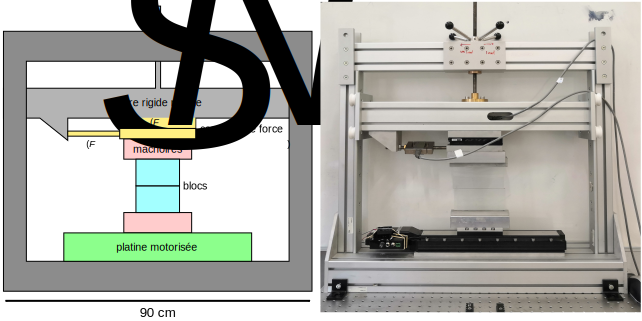
\includegraphics[scale=1]{../Figures_chap_exp/frame.pdf}
\caption[Schéma de la presse mécanique]{La presse est composée d'un cadre rigide (gris sombre), d'une barre horizontale mobile (gris clair), et d'une platine de translation commerciale (vert). La barre est installée par des poulies à gorge avec roulements à billes dans un guide limitant les rotations indésirables (roulis, tangage et lacet), et sa position est contrôlée manuellement par une vis. La platine de translation est contrôlable en position et en vitesse, pouvant aller de \SI{1}{\micro\meter\per\second} à \SI{10}{\mm\per\second}, sur une course de \SI{300}{\mm}. Des capteurs de forces (orange) permettent la mesure des forces normale et cisaillante appliquées à l'interface. Le dispositif est fixé par sa base sur une table optique.}
\label{fig:presse}
\end{figure}

\begin{figure}[h!]
\centering	
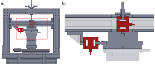
\includegraphics[scale=1]{../Figures_chap_exp/coupes_solidworks.pdf}
\caption[Disposition des capteurs de force]{\textbf{a.}\,Position des capteurs de force, en rouge, sur le cadre de la presse. Le capteur de force cisaillante est à gauche, le capteur de force normale est inséré dans la barre de translation verticale. \textbf{b.}\,Coupe transversale du cadre rouge. La force normale est appliquée sur l'interface au moyen d'une vis contrôlée manuellement, pressant sur le capteur de force. La force cisaillante est appliquée par le bloc inférieur, au moyen d'une platine de translation horizontale, et est retransmise au capteur de force cisaillante au moyen d'une platine à roulements à billes.}
\label{fig:captforce}
\end{figure}

\newpage


\section{Échantillons étudiés}
\label{sec:echantillons}

Nous avons étudié différents types d'interfaces frictionnelles, faisant intervenir des blocs solides et un système granulaire modèle, composés de matériaux plastiques.

Les blocs pressés sont des plaques fines de polyméthacrylate de méthyle de 80 mm de hauteur, formant une interface quasi bidimensionnelle de \qtyproduct[product-units=single]{150 x 10}{\mm}. Le milieu granulaire étudié est constitué de cylindres de nylon, de diamètre compris entre 0.4 et \SI{1.3}{\mm}, disposés dans la largeur de l'interface pour former un milieu granulaire 2D.

Cette section détaille les propriétés mécaniques des matériaux choisis pour les blocs et pour le milieu granulaire, ainsi que les géométries retenues pour notre étude.


\subsection{Blocs solides}

\subsubsection{Choix du matériau}
\label{sec:materials}

Le choix du matériau composant les plaques s'est fait sur le critère de la faible vitesse des ondes sonores en son sein, et donc de sa faible rigidité. En effet une plus grande rigidité implique une plus grande vitesse des ondes ($c_p\propto\sqrt{E/\rho}$), et impose une plus grande vitesse d'acquisition pour étudier les phénomènes propagatifs à l'interface. Pour autant nous utilisons un matériau suffisamment rigide pour ne pas atteindre son seuil de flambage. Notre choix s'est donc porté sur un matériau plastique rigide, le polyméthacrylate de méthyle (PMMA, ou \textit{Plexiglas}). Étant un matériau viscoélastique, son module d'Young $E$ dépend de la vitesse à laquelle il subit les déformations qui lui sont appliquées (il est dit \textit{strain rate dependent}\,\cite{mulliken_mechanics_2006}). Ainsi $E$ est compris entre 3.5 et \SI{5.6}{\giga\pascal} respectivement à faible et grande vitesse de sollicitation.

Afin de mesurer le module d'Young à l'aide de la presse, nous avons appliqué une force pressante sur un bloc de PMMA équipé de capteurs de déformation. Les mesures simultanées des déformations normale $\varepsilon_{yy}$ et orthogonale $\varepsilon_\perp$, et de la force normale $F_N$ appliquée sur la surface $A$ permettent de calculer $E$ et $\nu$ par un ajustement de la loi de Hooke (Fig.\,\ref{fig:fitE}). En effet $\sigma_{yy} = {F_N}/{A}=E\times\varepsilon_{yy}$ et $\nu = -{\varepsilon_\perp}/{\varepsilon_{yy}}$ (Sec.\,\ref{sec:hook}). Pour les chargements quasi-statiques, la valeur de $E$ mesurée et retenue est de \SI{3.5}{\giga\pascal}. Son coefficient de Poisson est $\nu = 0.3$. La vitesse des ondes de Rayleigh en son sein est $c_r\approx\SI{1250}{\meter\per\second}$. En référence, dans les métaux $E\approx\SI{100}{\giga\pascal}$ et $c_r\approx\SI{5000}{\meter\per\second}$, et dans les roches granitiques, $E\approx\SI{50}{\giga\pascal}$ et $c_r\approx\SI{2000}{\meter\per\second}$.

\begin{figure}[h!]
\centering	
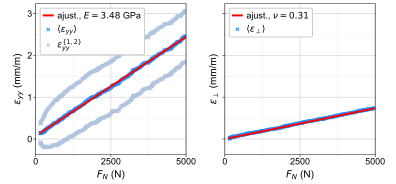
\includegraphics[scale=1]{../Figures_chap_exp/fit_E.pdf}
\caption[Mesure de $E$]{Mesure des propriétés mécaniques du PMMA. Le bloc de PMMA utilisé mesure \siprod{60 x 25 x 25}{\mm}, et est équipé de capteurs de déformation. La présence de deux capteurs de déformation sur des faces opposées permet de contrer leur non-parallélisme en effectuant la moyenne des deux mesures, c'est à dire $\left\langle\varepsilon_{yy}\right\rangle=(\varepsilon_{yy}^1+\varepsilon_{yy}^2)/2$.}
\label{fig:fitE}
\end{figure}






\subsubsection{Géométrie des blocs lisses}

La forme générale retenue pour les blocs est celle d'un parallélépipède de \siprod{150 x 80 x 10}{\mm}, en contact sur la tranche de \siprod{150 x 10}{\mm}. Les plaques sont rendues solidaires de la presse par le moyen de mors en acier de \SI{10}{\mm} de profondeur, ce qui réduit leur hauteur effective.

L'épaisseur du bloc a été choisie de \SI{10}{\mm}, faible devant ses deux autres dimensions, afin de pouvoir considérer l'échantillon comme bidimensionnel. Cette géométrie permet d'appliquer les simplifications associées à l'hypothèse de planéité des contraintes (\textit{plane stress}), et ainsi de restreindre le tenseur des déformations à deux dimensions et à trois composantes indépendantes. La face de contact a été dressée à la fraiseuse puis poncée manuellement avec du papier abrasif fin (P1200). La rugosité de surface de l'interface de contact est estimée à \SI{1}{\micro\meter} r.m.s. La planéité de la surface est de l'ordre de \SI{20}{\micro\meter}, mesurée avec un profilomètre confocal (Fig.\,\ref{fig:profilobloc}).


\begin{figure}[h]
\centering	
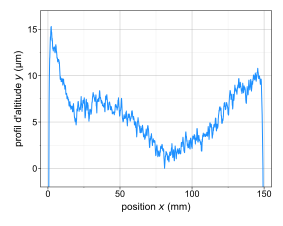
\includegraphics[scale=1]{../Figures_chap_exp/profil_bloc.pdf}
\caption[Profil moyen d'un bloc de PMMA]{Profil d'altitude moyen d'un des blocs pour l'étude d'une interface solide-solide, mesuré à l'aide d'un profilomètre confocal. La différence d'altitude entre le point le plus haut et le plus bas est de l'ordre de \SI{20}{\micro\meter} sur tous les blocs.}
\label{fig:profilobloc}
\end{figure}


\subsubsection{Géométrie des blocs granulaires}

\label{sec:geometriedesblocs}

Afin de solidariser le milieu granulaire aux blocs, le bord de ces derniers est percé d'alvéoles dans lesquelles des grains sont encastrés et collés (Fig.\,\ref{fig:blocgran}). Deux géométries sont alors utilisées dans notre étude, l'une que nous nommons l'interface en \textit{œil granulaire} et l'autre l'interface  \textit{entièrement granulaire}.


\myparagraph{Interface en œil granulaire}

L'interface en œil granulaire est composée de trois portions d'interface, deux portions solide-solide de 60 mm de long de part et d'autre d'un œil de longueur $\ell_{eye} = \SI{30}{\mm}$ contenant le milieu granulaire (Fig.\,\ref{fig:blocgran}a). L'œil est formé par deux cavités semi-elliptiques usinées dans chacun des blocs en contact, à la surface desquelles sont encastrés des grains de \SI{1.3}{\milli\meter} de diamètre tous les \SI{3}{\mm}. L'œil permet d'encapsuler un nombre variable de grains, faisant ainsi varier la densité du milieu. Le motif utilisé pour repérer optiquement les cylindres (Sec.\,\ref{sec:paint}) est reproduit en plusieurs points le long des portions solide-solide des blocs de part et d'autre de l'interface (Fig.\,\ref{fig:blocgran}c) afin de permettre des mesures de glissement interfacial (Sec.\,\ref{sec:suividesgrains}).


\pagebreak



\myparagraph{Interface entièrement granulaire}

L'interface entièrement granulaire est composée de grains dans toute sa longueur, encastrés dans le PMMA, soit à intervalle régulier, soit à intervalles aléatoirement générés, selon le bloc. Deux stoppeurs en silicone aux extrémités des deux blocs permettent de retenir une couche de grains d'épaisseur variable (\ref{fig:blocgran}b).




%\begin{figure}[h!]
\begin{figure}[htb]
\centering	
%\rule{0.6\textwidth}{0.4\textwidth}
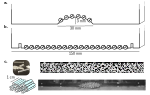
\includegraphics[scale=1]{../Figures_chap_exp/bloc_type_1.pdf}
\caption[Schéma des interfaces granulaires]{\textbf{a.}\,Interface à œil granulaire. L'œil granulaire mesure \SI{30}{\mm} de large par \SI{6}{\milli\meter} de hauteur et permet d'encapsuler une centaine de grains. \textbf{b.}\,Interface entièrement granulaire. Les grains encastrés à la surface du bloc sont espacés de 3 à \SI{8}{\milli\meter}, et peuvent être de diamètres variables. Les échelles ne sont pas respectées. \textbf{c.}\,Les grains sont disposés manuellement dans un arrangement aléatoire désordonné sur l'interface. Le motif peint sur les faces permet un suivi vidéo par corrélation d'images de la position et de la rotation de chaque grain, à une précision de l'ordre de \SI{5}{\micro\meter}.}
\label{fig:blocgran}
\end{figure}




\subsection{Milieu granulaire}

\myparagraph{Géométrie des grains}

Afin de conserver la structure quasi-bidimensionnelle du système, les grains sont des cylindres d'une longueur de \SI{10}{\milli\meter}, égale à la largeur de l'interface. Nous avons choisi des cylindres de différents diamètres (0.4, 0.7, 0.9 et \SI{1.3}{\milli\meter}) agencés parallèlement (Fig.\,\ref{fig:blocgran}c). La polydispersité des diamètres des grains permet d'éviter une cristallisation du milieu granulaire, qui modifierait ses propriétés mécaniques.




\myparagraph{Matériau des grains}

Les grains sont composés de Nylon ($E=\SI{1.4}{\giga\pascal}$, vérifié à l'aide d'une machine de traction, et $\nu=0.4$, tabulé), choisi pour ses propriétés mécaniques similaires à celles du PMMA composant les blocs. La proximité des modules d'Young des deux matériaux permet d'assurer un couplage entre l'élasticité de l'interface et celle des blocs.

Les cylindres sont réalisés à partir de fils de pêche de différents diamètres (0.4, 0.7, 0.9 et \SI{1.3}{\milli\meter}). Les fils sont redressés par la suspension d'une masse importante dans une étuve durant plusieurs heures. Une fois redressés ils sont manuellement coupés à la longueur voulue (\SI{10}{\milli\meter}) à l'aide d'une
%\href{https://youtu.be/hH5V2uqiSXc}{\textcolor{black}{guillotine}}
guillotine. Un motif est ensuite peint sur les deux faces circulaires des cylindres afin de faciliter le suivi des grains par imagerie (Sec.\,\ref{sec:paint}). L'état de surface du fil de nylon dans sa longueur n'est pas altéré.



Le système mécanique et les matériaux utilisés pour les échantillons ainsi définis, notre objectif est de mesurer les déformations des plaques minces de PMMA (\siprod{150 x 80 x 10}{\mm}, $E=\SI{3.5}{\giga\pascal}$) et les déplacements des grains de Nylon cylindriques (de diamètres allant de $0.4$ à \SI{1.3}{\mm}), afin de caractériser le comportement des différentes interfaces (surface lisse, entièrement granulaire ou en œil granulaire) que nous souhaitons étudier. Pour ce faire, nous avons développé un système de mesure électronique, reposant sur l'utilisation de jauges de déformation, et un système optique utilisant des méthodes de suivi par corrélation d'image.





\section{Mesures Électroniques}
\label{sec:electronique}

Afin de caractériser les efforts macroscopiques appliqués sur l'interface et leur répartition locale, ainsi que la dynamique des ruptures associées aux évènements de glissement, nous avons développé un système électronique permettant de mesurer les déformations des blocs et les forces pressante et cisaillante qui leur sont appliquées.

Le système électronique que nous avons développé, en partenariat avec Pascal Metz et Julian Miniot du Service d'Ingénierie Électronique du Laboratoire de Physique à l'ENS de Lyon, est une évolution du circuit développé dans le groupe de J. Fineberg (Hebrew University of Jerusalem).
Il permet d'amplifier et d'acquérir 60 voies de tension simultanément. Il combine des rafales d'acquisition rapide de \SI{10}{\milli\second} à \SI{4}{\mega\hertz}, déclenchées par un signal accélérométrique, et une acquisition lente à \SI{315}{\hertz} pouvant durer plusieurs dizaines de minutes. Il nous permet d'acquérir le signal de jauges de déformation, fournissant ainsi une mesure du tenseur des déformations 2D en 20 points le long de l'interface, ainsi que le signal des capteurs de forces normale et cisaillante, et du détecteur d'évènements accélérométrique.

Cette section détaille le dispositif de mesure des déformations et des forces, et de détection d'évènements.


\subsection{Mesure du tenseur des déformations}

La connaissance complète du tenseur des déformations 2D $[\varepsilon]$ permet de déterminer de nombreuses informations, telles que la répartition de la charge le long de l'interface, la vitesse et la direction de propagation des ondes, et les propriétés des ruptures interfaciales\,\cite{svetlizky_brittle_2017}. Ainsi mesurer $\varepsilon$ avec précision et à haute fréquence est l'objet principal du développement électronique que nous avons effectué. Sa mesure repose sur l'utilisation, le conditionnement, l'amplification et l'acquisition du signal de jauges de déformation.

\subsubsection{Jauge de déformation}
\label{sec:gages}

\myparagraph{Fonctionnement}

Une jauge de déformation est une feuille métallique de résistance connue, disposée en forme de créneau, intégrée dans une matrice en matériau isolant (Fig.\,\ref{fig:jauge}a). Elle est installée à l'aide d'un adhésif spécifique qui solidarise la matrice à la surface de l'échantillon étudié. Cette colle permet à toutes les déformations de l'échantillon d'être retransmises à la résistance, qui se déforme avec le bloc et voit sa valeur changer.

La variation de résistance est reliée à la déformation mécanique qu'elle subit dans son axe, notée $\varepsilon_{\parallel}$, par une loi polynomiale. Cette loi est généralement tronquée en une réponse linéaire par un coefficient $GF$ nommé \textit{facteur de jauge}, d'une valeur typique de l'ordre de 2, selon l'équation suivante, où $R_r$ est la résistance de la jauge au repos, et $\delta R$ est l'écart à cette valeur :

\begin{equation}
\label{eq:jauge}
\dfrac{\delta R}{R_r} = GF\times \varepsilon_{\parallel}
\end{equation}

Ainsi la mesure d'une déformation uni-axiale consiste en la mesure précise des variations d'une résistance.



Les jauges que nous utilisons sont agencées en rosettes à trois jauges (Fig.\,\ref{fig:jauge}b), écartées d'un angle de \ang{45}, de résistance \SI{350 +- 2}{\ohm}, et de facteur de jauge $GF=1.86$ pour les deux jauges latérales de la rosette, et $GF=1.79$ pour la jauge centrale de la rosette.



\begin{figure}[htb]
\centering	
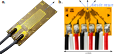
\includegraphics[scale=1]{../Figures_chap_exp/jauges.pdf}
\caption[Jauge de déformation]{\textbf{a.}\,Une jauge de déformation uni-axiale. Un allongement (respectivement une contraction) de sa matrice dans le plan provoque un allongement et un affinement par contraction de Poisson (resp. raccourcissement et épaississement) de la feuille métallique. Ces deux effets entraînent une augmentation (resp. diminution) de la valeur de la résistance. \textbf{b.}\,Trois jauges disposées en rosette, modèle utilisé dans notre étude. Lorsqu'une mesure bidimensionnelle du tenseur des déformations est requise, les jauges sont agencées en rosette dans une même matrice, permettant ainsi d'obtenir les trois composantes du tenseur 2D.}
\label{fig:jauge}
\end{figure}


\myparagraph{Nécessité d'amplifier -  calcul d'ordre de grandeur}

La variation de résistance $\delta R$ induite par les déformations du bloc est très faible par rapport à la valeur de résistance au repos $R_r$ de la jauge. Un calcul d'ordre de grandeur de la valeur de $\delta R$ dans le cadre typique de notre étude permet de déterminer la précision requise pour mesurer le signal de la jauge de déformation.

Prenons une force constante de 3000 N appliquée sur une interface de $150\times10$ mm, soit une surface \SI{1.5e-3}{\square\meter}, dans un bloc de PMMA de module d'Young $E=\SI{4}{\giga\pascal}$, parallèlement à l'axe d'une jauge de déformation de résistance $R_r=\SI{350}{\ohm}$ et de facteur de jauge $GF=2$. Alors la contrainte est donnée par
$\sigma_{\parallel} = {F_N}/{A} = \SI{2}{\mega\pascal}$. La loi de Hooke stipule que $\sigma_{\parallel}=E\varepsilon_{\parallel}$, donnant $\varepsilon_{\parallel} = \qty[per-mode = symbol]{5e-4}{\meter\per\meter}$. Enfin $\delta R/R_r = GF\times \varepsilon_{\parallel}$ permet de retrouver $\delta R =\SI{350}{\milli\ohm}$. Pour mesurer la composante continue du tenseur des déformations à \SI{10}{\percent} près, il faut donc pouvoir résoudre une valeur constante de l'ordre de \SI{10}{\milli\ohm}.

Si maintenant l'on considère une rupture typique issue de la théorie de la Mécanique de la Fracture Élastique Linéaire (LEFM, Sec.\,\ref{sec:LEFM}) d'énergie de rupture $\Gamma=\SI{1}{\joule\per\meter\squared}$, une vitesse de \SI{500}{\meter\per\second}, et des jauges installées à \SI{3}{\milli\meter} de l'interface, et que l'on calcule la variation typique de $\varepsilon_{\parallel}$ à son passage, nous trouvons que $\delta\varepsilon_{\parallel}\approx\qty[per-mode = symbol]{5e-5}{\meter\per\meter}$, et une variation de résistance associée de $\delta R = \SI{35}{\milli\ohm}$. Ainsi nous avons besoin d'une résolution de l'ordre du milliohm pour mesurer l'évolution de la composante variable du tenseur des déformations à $10^{-5}\,\text{m}/\text{m}$ près.

Pour mesurer ces faibles variations plusieurs approches existent, mais toutes sont équivalentes à mesurer une variation de la tension $U$ aux bornes de la jauge à intensité $I$ fixée. En notant $U=U_r+\delta U$, avec $U_r=R_r\times I$, sous obtenons

\begin{equation}
\delta U = \delta R\times I = GF\times R_r\times I\times \varepsilon_{\parallel}
\label{eq:1.2}
\end{equation}

Plus l'intensité sera élevée, plus les variations de tensions $\delta U$ seront élevées. 


Cependant les jauges étant des conducteurs ohmiques, elles dissipent une puissance $\mathcal{P}=U\times I=R I^2$ en chaleur, et peuvent fondre si cette chaleur n'est pas évacuée suffisamment rapidement. Le choix d'un matériau plastique, de faible conductivité thermique, limite grandement cette possibilité de dissipation ($\lambda_{\mathrm{PMMA}}\approx \SI{0.2}{\watt\per\meter\per\kelvin}$, en comparaison pour un matériau métallique $\lambda_{\mathrm{metal}}\sim 10^2\,\unit{\watt\per\meter\per\kelvin}$). La puissance dissipable est au maximum de \SI{1}{\milli\watt}, ce qui correspond à un courant d'intensité $I=\SI{1.7}{\milli\ampere}$.

La différence d'échelle entre la tension au repos $U_r$ et la variation de tension $\delta R$ soulève une autre difficulté. En effet à cette intensité de courant $U_r\approx\SI{0.6}{\volt}$, et si l'on conserve le critère de résolution de $10^{-5}$ m/m pour le tenseur des déformations, $\delta U\approx\SI{1}{\micro\volt}$. Ainsi une tentative d'amplification directe du signal de jauge est impossible, puisque l'amplification de la composante continue écraserait le signal à mesurer.

Pour mesurer cette tension, la technique expérimentale la plus couramment utilisée est le conditionnement par un pont de Wheatstone. Bien que nous ayons décidé à terme de ne pas utiliser de pont de Wheatstone dans le conditionnement de nos jauges de déformation mais une amplification par boucle d'Anderson, la présentation de ce montage permet d'en comprendre les avantages et les limites, et de justifier notre choix.

\subsubsection{Conditionnement traditionnel par pont de Wheatstone}


Un pont de Wheatstone est un circuit électrique pouvant être utilisé pour déterminer la valeur d'une résistance électrique inconnue, et pour mesurer avec précision ses fluctuations autour d'une valeur d'équilibre. Ce montage permet non seulement de mesurer avec précision la résistance d'une jauge, mais aussi ses variations autour de son état au repos, dans la limite de faibles écarts.



\begin{figure}[htb]
\centering	
\includegraphics[scale=1]{../Figures_chap_exp/Wheatstonebridge.pdf}
\caption[Pont de Wheatstone]{Montage d'un pont de Wheatstone en configuration quart-de-pont. Une des résistances du pont est une jauge de déformation, tandis que les trois autres sont des résistances fixes de valeur $R=R_r$ égale à la résistance au repos de la jauge. En pratique, afin de pallier aux variations de résistance des composants autour de leur valeur nominale et d'équilibrer le pont, la résistance $R_{\mathrm{BD}}$ est un potentiomètre. La tension $U_{\mathrm{AB}}$ est fixée constante, et la tension mesurée est la tension $U_{\mathrm{CD}}$.}
\label{fig:wheatstone}
\end{figure}


\myparagraph{Principe}


 En utilisant le théorème de Millman sur le montage présenté (Fig.\,\ref{fig:wheatstone}) nous obtenons
 
\begin{equation}
U_{\mathrm{CD}} = U_{\mathrm{AB}}
	\times
\dfrac{\delta R}{4R_r}
	\times
\left(
	\dfrac{1}{1+\frac{\delta R}{4R_r}}
\right)
\end{equation}

De plus, la fonction $f$ qui à $x$ associe $f(x)=\dfrac{1}{1+x}$ étant de classe $\mathcal{C}^\infty$ autour de 0, le théorème de Taylor-Young assure qu'il existe un développement limité de cette fonction en 0, et que ce développement limité prend la forme

\begin{equation}
f(x) = f(0) + f'(0)\times x + \dfrac{f''(0)}{2!}\times x^2 +\dots+  \dfrac{f^{(n)}(0)}{n!}\times x^n  + o(x^n)
\end{equation}

Étant donné que dans les conditions normales d'utilisation d'une jauge de déformation ${\delta R}/{4R_r}$ est proche de 0,  nous pouvons appliquer ce développement limité à $U_{\mathrm{CD}}$, avec $x={\delta R}/{4R_r}$ et $n=3$, ce qui donne

\begin{equation}
U_{\mathrm{CD}}= \dfrac{U_{\mathrm{AB}}}{4}
	\times
\left[
	\dfrac{\delta R}{R_r}
		-
	\dfrac{1}{4}\left(\dfrac{\delta R}{R_r}\right)^2
		+
	\mathcal{O}
		\left(
			\left(\dfrac{\delta R}{R_r}\right)^3
		\right)
\right]
\end{equation}

Et en utilisant la relation résistance-déformation d'une jauge (Éq.\,\ref{eq:jauge}) il vient

\begin{equation}
U_{\mathrm{CD}}= \dfrac{U_{\mathrm{AB}}}{4}
	\times
\left[
	GF\times\varepsilon_{\parallel}
		-
	\dfrac{1}{4}\left(GF\times\varepsilon_{\parallel}\right)^2
		+
	\mathcal{O}
		\left(
			\left(GF\times\varepsilon_{\parallel}\right)^3
		\right)
\right]
\end{equation}

Ce développement est ensuite généralement tronqué à l'ordre 1, donnant

\begin{equation}
U_{\mathrm{CD}}= \dfrac{U_{\mathrm{AB}}\times GF}{4} \times \varepsilon_{\parallel} +
	\mathcal{O}\left( \varepsilon_{\parallel}^2 \right)
\end{equation}



Cette expression montre que le pont de Wheatstone permet de s'affranchir de la contrainte posée par la composante continue $U_r$ décrite au paragraphe précédent. Une amplification du signal d'intérêt tel quel est possible, mais sacrifie la linéarité de la réponse en tension de la jauge.


\myparagraph{Potentielles limites du pont de Wheatstone}


L'apparition d'une non-linéarité constitue une des limites théoriques du pont de Wheatstone, mais n'a en pratique pas d'influence dans le cadre de notre étude. En effet, en reprenant les valeurs typiques données plus haut (Éq.\,\ref{eq:1.2}), nous pouvons évaluer la contribution du premier terme non-linéaire comme $10^{4}$ fois plus petite que celle du terme linéaire pour la composante variable de la valeur de résistance. Cela justifie de négliger son apport et celui des termes suivants dans le développement limité.


Une difficulté technique posée par un pont de Wheatstone réside dans l'équilibrage du pont. Nous avons supposé pour les calculs précédents que les trois résistances sont de même valeur $R=R_r$ que la jauge au repos, mais les résistances commerciales usuelles, ainsi que les jauges, ont des tolérances de l'ordre de quelques pourcents. Ces variations de résistance doivent être compensées en équilibrant le pont à l'aide d'un potentiomètre. Si nous nommons $\Delta_{\mathrm{C}} = R_{\mathrm{AC}}-R_{\mathrm{BC}}$ et $\Delta_\mathrm{D} = (R_{\mathrm{AD}} - \delta R)  - R_{\mathrm{BD}} = R_r - R_{\mathrm{BD}}$, alors nous pouvons écrire au premier ordre en $\Delta_{\mathrm{C}}$ et $\Delta_\mathrm{D}$

\begin{equation}
U_{\mathrm{CD}} = \dfrac{U_{\mathrm{AB}}}{4}\times\left[\dfrac{\Delta_\mathrm{D} + \delta R}{R_{\mathrm{BD}}}-\dfrac{\Delta_{\mathrm{C}}}{R_{\mathrm{BC}}}\right]
\end{equation}

Ainsi si les résistances $R_{\mathrm{AC}}$ et $R_{\mathrm{BC}}$ n'ont pas la même valeur, la tension mesurée subit un décalage proportionnel à cet écart. Ce décalage doit être compensé par un potentiomètre, installé à la position $\mathrm{BD}$, de sorte à ce que $\Delta_\mathrm{D}/R_{\mathrm{BD}} = \Delta_\mathrm{C}/R_{\mathrm{BC}}$. Alors nous obtenons

\begin{equation}
U_{\mathrm{CD}} = \dfrac{U_{\mathrm{AB}}}{4}\times\dfrac{\delta R}{R_{\mathrm{BD}}}
\end{equation}

Dans le cas de résistances ayant une tolérance de \SI{2}{\percent}, cette variation de $R_{BD}$ peut mener jusqu'à \SI{0.1}{\percent} de variation sur $U_{CD}$. Cet effet est faible, mais supérieur (et non-exclusif) à celui de la non-linéarité.


Enfin un conditionnement par pont de Wheatstone soulève également d'autres difficultés pratiques, telles que la prise en compte de la longueur des fils et de leur sensibilité au bruit. D'autres montages dits \textit{demi-pont} ou \textit{pont complet} permettent de contourner ces effets, mais sont plus complexes à mettre en place, nécessitant notamment l'installation de plusieurs jauges par point de mesure. Pour ces raisons, nous avons opté pour un système électronique au principe différent, la boucle d'Anderson.

\subsubsection{Boucle d'Anderson}
\label{sec:anderson}

\begin{figure}[htb]
\centering	
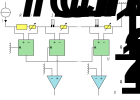
\includegraphics[scale=1]{../Figures_chap_exp/anderson_schema_reversed.pdf}
%\includegraphics[width=.2\textwidth]{../Figures_chap_exp/anderzoom.png}
\caption[Boucle d'Anderson]{Schéma électrique de la boucle d'Anderson. La boucle d'Anderson repose sur une boucle de jauges en série avec une résistance de référence, et deux étages d'amplification successifs. Le premier étage amplifie le signal brut des jauges (composante continue comprise) par un faible gain $\mathrm{G}_1$, et soustrait à chaque signal de jauge ainsi amplifié une tension de référence. Pour ce faire, une résistance de référence est ajoutée à la boucle, et la tension à ses bornes est amplifiée par le même gain que les jauges, mais sans soustraction. Le signal de référence amplifié est ensuite soustrait à tous les autres, dans chaque amplificateur de la boucle. Le deuxième étage est un amplificateur de grand gain $\mathrm{G}_2$. Des potentiomètres sont installés en série avec chaque jauge pour compenser les légères variations dans les valeurs de $R_r$ entre les jauges.}
\label{fig:anderson}
\end{figure}



\myparagraph{Principe}


La boucle d'Anderson\,\cite{anderson_nasas_1998} repose sur le principe de mettre en série à intensité $I$ constante plusieurs jauges $J_i$ de valeur au repos $R_r$, ainsi qu'une résistance de référence de valeur $R_r$ constante, et d'utiliser cette dernière pour éliminer la composante au repos des jauges. La tension $U_r$ aux bornes de la résistance de référence est soustraite aux tensions des jauges par un composant actif. La tension résultante est ensuite amplifiée par deux étages d'amplification successifs de gains $\mathrm{G}_1$ et $\mathrm{G}_2$, pour permettre l'acquisition du signal. Le schéma électrique de principe est détaillé en Figure\,\ref{fig:anderson}.



Si nous considérons une des jauges du circuit, et nommons $V_+$ et $V_-$ les potentiels à ses bornes, alors le signal en sortie du premier étage vaut

\begin{equation}
U_1=\mathrm{G}_1\times(V_+-V_-)-\mathrm{G}_1\times U_r
\end{equation}

En prenant en compte que $V_+-V_- = (R_r+\delta R)\times I$ et $U_r=R_r\times I$, nous obtenons

\begin{equation}
U_1=\mathrm{G}_1\times\delta R \times I
\end{equation}

Ainsi le premier étage élimine bien la composante au repos du signal des jauges.

Le signal en sortie du deuxième étage vaut

\begin{equation}
U_2=\mathrm{G}_2\times U_1=\mathrm{G}_1\times \mathrm{G}_2\times\delta R\times I
\end{equation}

Le signal de sortie s'exprime comme une fonction linéaire de $\delta R$, et donc de $\varepsilon_{\parallel}$.


La résistance de référence peut être physiquement déportée et positionnée proche de l'échantillon et des jauges de déformation. Elle a alors une résistance fixe mais est dans le même environnement électromagnétique que les autres jauges (longueur de câble, position, orientation, etc.). Ainsi si les jauges subissent un champ électromagnétique fort (bruit coloré, néons, signaux téléphoniques, etc.), la proximité de la référence permet d'annuler tout signal parasite par la soustraction effectuée dans le premier étage d'amplification. Afin de rendre les environnements électromagnétiques des jauges et de la référence plus proches encore, il est possible d'utiliser une jauge non solidaire du bloc pour remplir le rôle de référence.

La boucle d'Anderson dispose donc en théorie de nombreux avantages, en particulier sa linéarité exacte, sa relative simplicité de réglage, et sa capacité à résister au bruit. C'est pour cela que nous avons choisi de l'implémenter dans notre dispositif électronique. Cependant cette méthode fait intervenir une soustraction active et plusieurs étages d'amplification, pouvant générer du bruit.



\myparagraph{Mise en pratique -  évaluation du bruit}



\begin{figure}[htb]
\centering	
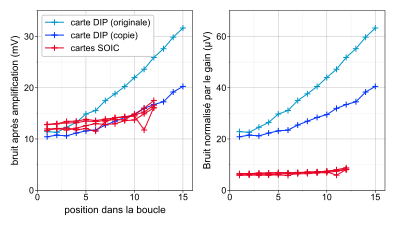
\includegraphics[scale=1]{../Figures_chap_exp/test_JPBox_fast.pdf}
\caption[Niveau de bruit dans nos dispositifs d'amplification]{Comparaison du niveau de bruit (écart type d'un signal à vide) entre les deux systèmes d'amplification. Les deux cartes du premier jeu, en bleu, génèrent un bruit croissant avec la distance de la jauge à la source de courant, témoignant d'une fuite de courant. Les 5 cartes du deuxième jeu, en rouge, bien qu'ayant un niveau de bruit brut à première vue similaire à celles du premier jeu, ont un niveau de bruit 4 fois moins grand une fois normalisé par le gain, et ce malgré une bande passante plus élevée. Leur fuite de courant est beaucoup plus faible, comme montré par la faible différence de niveau de bruit entre la première et la dernière jauge de la boucle.}
\label{fig:bruit}
\end{figure}




Lors de notre étude, nous avons fabriqué et utilisé deux jeux de circuits imprimés différents, implémentant chacun une boucle d'Anderson avec une approche différente, le deuxième ayant été dessiné et fabriqué pour combler les lacunes du premier. Les performances des deux systèmes sont comparées en Figure\,\ref{fig:bruit}.


\myparagraph{Premier jeu de cartes -- DIP}

Le premier jeu de cartes, utilisé dans cette étude jusqu'en janvier 2024, est adapté d'un circuit déjà existant, utilisé dans le groupe de J. Fineberg au \textit{Racah Institute of Physics} de la \textit{Hebrew University of Jerusalem}, conçu en 2012. Chaque carte consiste en une boucle de 15 jauges et d'une référence, avec deux étages d'amplification de gains $10\times50$. La bande passante de ce système est de \SI{500}{\kilo\hertz} (produit gain bande de $2.5\times10^8$). Nous avons utilisé en parallèle deux cartes de 15 voies, soit 30 jauges agencées en 10 rosettes, permettant 10 points de mesure simultanée à l'interface.

Ce jeu de cartes a plusieurs limitations intrinsèques à sa conception. Tout d'abord les amplificateurs utilisés sont des composants DIP (\textit{Dual Inline Package}), ce qui augmente l'espace physique occupé par les cartes, la quantité de chaleur dissipée par le système, et le niveau de bruit. De plus chaque amplificateur représente une fuite de courant, et ajoute du bruit dans le courant reçu par la jauge suivante. Le niveau de bruit augmente ainsi tout le long de la boucle jusqu'à masquer le signal. Cette dernière limitation est d'autant plus marquée que le circuit a initialement été développé pour des jauges de \SI{120}{\ohm}, et que nous l'utilisons avec des jauges de \SI{350}{\ohm}. Pour cette raison, la deuxième carte du jeu DIP est une copie légèrement remaniée de la première et son niveau de bruit en est réduit (Fig.\,\ref{fig:bruit}).


%%%%%%%%%%

En raison des limitations techniques de ce système, nous avons développé au long de notre étude un deuxième jeu de cartes, dont la conception a été finalisée en janvier 2024.


\myparagraph{Deuxième jeu de cartes -- SOIC}

Le deuxième jeu est composé de 5 boucles contenant chacune 12 jauges et une référence, ayant un gain de $10\times200$. La bande passante de ce système est de \SI{5}{\mega\hertz} (produit gain bande de $10^{10}$). Les 5 cartes sont insérées dans un unique boîtier blindé de format 2U.

Afin de combler les lacunes du système précédent, nous avons utilisé des composant SOIC (\textit{Small Outline Integrated Circuit}) plus récents et performants. Les circuits d'amplification sont équipés de nombreux filtres capacitifs et de ferrites limitant le bruit d'amplification et stabilisant l'alimentation, ainsi que de composants de haute impédance limitant les fuites de courant. Ces améliorations nous ont permis de réduire d'un facteur 3 à 8 l'écart type du bruit électronique normalisé par le gain par rapport au premier jeu de cartes (Fig.\,\ref{fig:bruit}).






\subsubsection{Reconstruction du tenseur des déformations 2D}



\begin{figure}[htb]
\centering	
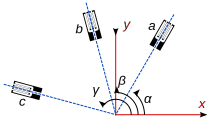
\includegraphics[scale=1]{../Figures_chap_exp/StrainRosetteAngles.pdf}
\caption[Reconstruction du tenseur des déformations]{Notations des angles dans une rosette à trois jauges de déformation. Les capteurs que nous utilisons sont des rosettes à trois jauges, écartées d'un angle de \ang{45} de part et d'autre de l'axe $y$, nommé axe principal de la rosette ($\alpha=\beta=\gamma=\ang{45}$). Dans notre étude, cet axe est disposé perpendiculairement à l'interface.}
\label{fig:anglerosette}
\end{figure}





Les jauges de déformation permettent des mesures de déformation uni-axiales, cependant nous cherchons à mesurer le tenseur des déformations complet à l'interface. Il est possible de reconstruire ce tenseur en utilisant 3 jauges de déformation disposées en rosette.

La géométrie du système permet de réduire le tenseur $[\varepsilon]$ à deux dimensions

\begin{equation}
{[\varepsilon]}
=
\begin{bmatrix}
	\varepsilon_{xx} & \varepsilon_{xy} \\
	\varepsilon_{xy} & \varepsilon_{yy}
\end{bmatrix}
\end{equation}
 

Pour calculer les composantes $\varepsilon_{xx}$, $\varepsilon_{xy}$ et $\varepsilon_{yy}$ du tenseur des déformations à partir de trois mesures non-coaxiales des déformations du bloc $\varepsilon_{\{a,b,c\}}$ (Fig.\,\ref{fig:anglerosette}) nous utilisons l'expression suivante :


\begin{align}[left=\empheqlbrace]
\begin{split}
		\varepsilon_a
	&=
		\dfrac{\varepsilon_{xx}+\varepsilon_{yy}}{2}+\dfrac{\varepsilon_{xx}-\varepsilon_{yy}}{2} \cos( 2 \alpha)+\varepsilon_{xy} \sin (2 \alpha)
	\\
		\varepsilon_b
	&=
		\dfrac{\varepsilon_x+\varepsilon_y}{2}+\dfrac{\varepsilon_x-\varepsilon_y}{2} \cos (2(\alpha+\beta))+\varepsilon_{x y} \sin (2(\alpha+\beta))
	\\
		\varepsilon_c
	&=
		\dfrac{\varepsilon_x+\varepsilon_y}{2}+\dfrac{\varepsilon_x-\varepsilon_y}{2} \cos (2(\alpha+\beta+\gamma))+\varepsilon_{x y} \sin (2(\alpha+\beta+\gamma))
\end{split}
\end{align}

Ainsi dans le cas d'une rosette de trois jauges écartées de \ang{45}, et dont l'axe de la jauge centrale est l'axe $y$, il vient

\begin{align}[left=\empheqlbrace]
\label{eq:rotation}
\begin{split}
		\varepsilon_{xx}
	&=
		\varepsilon_{a}-\varepsilon_{b}+\varepsilon_{c}
	\\
		\varepsilon_{yy}
	&=
		\varepsilon_{b}
	\\
		\varepsilon_{xy}
	&=
		\left(\varepsilon_{a}-\varepsilon_{c}\right)/2
\end{split}
\end{align}




\subsubsection{Disposition des jauges sur les blocs}


Le choix que nous avons effectué pour la plupart des expériences présentées est de disposer d'un côté du bloc une rosette tous les centimètres tout le long de l'interface, soit 15 rosettes, et 5 rosettes sur l'autre face, servant à contrôler la symétrie des contraintes appliquées. Les jauges d'intérêt ont ensuite été choisies en fonction des besoins de chaque expérience et des capacités du dispositif d'amplification utilisé. Les rosettes sont disposées à \SI{2 +- 0.2}{\milli\meter} de l'interface, permettant d'avoir un signal important au passage d'une rupture.
%tout en restant hors de la zone de régularisation des contraintes
Leur axe principal (Fig.\,\ref{fig:anglerosette}) est disposé perpendiculairement à l'axe de l'interface.


\subsection{Acquisition}


\subsubsection{Spécifications des acquisitions}

Le système d'acquisition dispose de 64 voies, dont 60 correspondent aux 60 jauges (20 rosettes) conditionnées par le système d'amplification, connectées par un connecteur blindé dédié. Les 4 autres voies sont accessibles par un connecteur coaxial standard, et peuvent servir à mesurer diverses observables. Dans notre étude, 2 de ces voies sont dédiées aux capteurs de forces normale et cisaillante, et une à un déclenchement accélérométrique, détaillé plus bas. Une voie est laissée libre pour de futures applications.

Un évènement de rupture typique durant de l'ordre d'une milliseconde (Sec.\,\ref{sec:LEFM}), les canaux sont acquis par salves de \SI{10}{\milli\second} à une fréquence d'acquisition de \SI{4}{\mega\hertz}, déclenchées par un accéléromètre. Cette acquisition rapide est doublée d'une acquisition lente, à \SI{315}{\hertz}, en continu sur une expérience. Les signaux acquis sont numérisés sur 14 bits avec un suréchantillonnage à \SI{40}{\mega\hertz}, sur une plage de tension d'entrée de [-4, 4] V, donnant une résolution de $10^{-5}\,\text{V}$.


\subsubsection{Déclenchement par accéléromètre}
\label{sec:accel}

Afin de détecter les évènements de glissement rapide de l'interface, et de donner un signal de déclenchement aux acquisitions rapides, nous utilisons un accéléromètre collé sur le bord d'un des blocs. L'accéléromètre agit comme un sismomètre et reçoit les ondes émises au moment d'un évènement de glissement. Son signal est généré par effet piézoélectrique, passif, et est d'une très faible puissance. Il doit donc être amplifié, puis converti en signal de logique transistor (TTL).

Le circuit d'amplification (Fig.\,\ref{fig:accel}) est composé d'un système d'amplification de grand gain réglable (jusqu'à 500). La sortie de l'amplificateur est connectée à l'entrée de deux multivibrateurs monostables en série. Un multivibrateur monostable est un composant électronique qui émet une impulsion TTL de longueur définie lorsque son entrée dépasse un seuil fixé. Ainsi un évènement de glissement va entraîner un déclenchement des deux multivibrateurs, et l'émission de deux impulsions TTL, une courte (quelques microsecondes) et une longue (quelques millisecondes), utilisées respectivement comme déclencheur de l'acquisition rapide et comme repère d'évènement de glissement dans l'acquisition lente.






\subsection{Traitement numérique des données acquises}
\label{sec:electroniquedonnées}

Les données brutes fournies par le boîtier d'acquisition sont converties en valeurs de tension, enregistrées en nombres flottants sur 64 bits, sous le langage de programmation Python3 (\texttt{<class 'numpy.float64'>}), permettant une précision de l'ordre de 16 chiffres significatifs. Le même langage est utilisé pour tous les traitements ultérieurs. Les données d'acquisition électronique sont rassemblées avec les données optiques (Sec.\,\ref{sec:optiquesdonnées}), et les traitements finaux et figures sont réalisés sous Python3\,\cite{van_rossum_python_2009, harris_array_2020,hunter_matplotlib_2007}.

Afin d'éliminer l'erreur systématique induite par le réglage des potentiomètres des jauges sur la valeur de tension mesurée, une valeur de référence prise avec les capteurs à vide lui est soustraite. La disposition des jauges est contrôlée en passant chaque bloc dans un scanner de documents à haute résolution. Ainsi la distance à l'interface des rosettes est vérifiée, et  la rotation de chacune peut si besoin être prise en compte et corrigée lors de la reconstruction du tenseur des déformations (Éq.\,\ref{eq:rotation}).

Nous avons également implémenté des méthodes numériques de réduction de bruit telles que des filtres, utilisées dans divers traitements de données et pour certaines représentations graphiques. Nous avons principalement utilisé des filtres passe-bas sous la forme de moyennes glissantes, mais aussi plus anecdotiquement des filtres passe-bande et coupe-bande, pour caractériser et éliminer des bruits colorés.


\newpage



\begin{figure}[h!]
\centering	
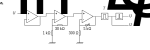
\includegraphics[scale=1]{../Figures_chap_exp/trigger.pdf}\\
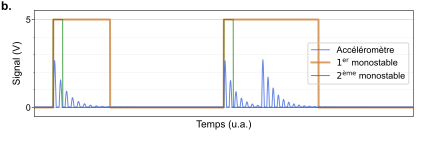
\includegraphics[scale=1]{../Figures_chap_exp/signal_accelero.pdf}
\caption[Système de déclenchement accélérométrique]{\textbf{a.}\,Schéma électrique du conditionnement de l'accéléromètre. Le circuit d'amplification se décompose successivement en un suiveur de grande impédance, un amplificateur de gain fixe, un amplificateur réglable, un multivibrateur monostable re-déclenchable à longue pulsation, puis enfin un multivibrateur monostable non re-déclenchable à pulsation courte. Cette combinaison permet de détecter les évènements de glissement, en passant outre les oscillations macroscopiques du système.  \textbf{b.}\,Représentation simplifiée de signaux réels. En bleu, un signal typique correspondant à l'accéléromètre amplifié. En ocre, la sortie du premier multivibrateur. En vert, la sortie du deuxième.}
\label{fig:accel}
\end{figure}



\vspace{10mm}

\section{Mesures Optiques}
\label{sec:optique}

En parallèle de l'acquisition électronique, nous imageons la surface des blocs à l'aide d'une caméra rapide. Cela nous permet un suivi optique autour de l'interface, et la mesure des déplacements des grains par corrélation d'images, à une précision de l'ordre de \SI{5}{\micro\meter}. Cette section détaille l'optique utilisée et les méthodes numériques implémentées pour l'analyse des images.

\subsection{Optique utilisée}

L'acquisition optique est réalisée à l'aide d'une caméra rapide Phantom V2511 pouvant aller de 100\,fps à 1\,Mfps. La caméra est équipée selon les besoins d'objectifs dont la focale varie de 85 à \SI{135}{\milli\meter}. La résolution maximale du capteur est de $1280\times800$ pixels, mais il est possible de n'utiliser qu'une portion du capteur, ce qui permet d'augmenter la vitesse d'acquisition. Nous avons principalement utilisé le capteur dans toute sa largeur pour filmer tout le long de l'interface à 100 ou 1\,000\,fps, mais des tests préliminaires ont été effectués jusqu'à 500 kfps.

L'acquisition peut être déclenchée par le même accéléromètre que celui utilisé pour le dispositif d'acquisition électronique.


\newpage

\subsection{Suivi des grains - recherche de motif}
\label{sec:suividesgrains}

La recherche de motif dans une image (\textit{template matching}) permet de trouver la position la plus probable d'un motif de référence donné dans une image le contenant. Un exemple emblématique de recherche de motif est la reconnaissance de texte, dans lequel les caractères d'écriture servent de motif de référence à chercher. Nous l'avons pour notre part utilisé pour détecter et suivre la position des cylindres à l'interface.




\subsubsection{Détermination des motifs à suivre par transformée de Hough}
\label{sec:paint}



\begin{figure}[htb]
\centering	
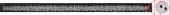
\includegraphics[scale=1]{../Figures_chap_exp/fullygran_zoom.pdf}
\caption[Interface entièrement granulaire]{Photographie de l'interface entièrement granulaire. Les cylindres sont déposés à l'interface et font face à la caméra. Leur face plane est blanche avec deux points noirs.}
\label{fig:facegrains}
\end{figure}



\begin{figure}[htb]
\centering	
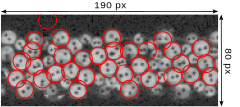
\includegraphics[scale=1]{../Figures_chap_exp/correlation_grains_0.pdf}
\caption[Détection des grains par transformée de Hough]{Détection initiale de la position des cylindres. Cette détection, effectuée par transformée de Hough, est corrigée manuellement pour éliminer les faux positifs et rajouter les cylindres non détectés.}
\label{fig:hough}
\end{figure}



Les cylindres sont disposés de telle sorte à ce que leur face circulaire soit contenue dans le plan filmé par la caméra, pour permettre de suivre leur mouvement en deux dimensions. Afin d'améliorer le contraste des images et la reconnaissance des faces, nous les avons peintes en blanc, et dessiné deux points noirs pouvant également servir à suivre leur rotation (Fig.\,\ref{fig:facegrains}). Les cylindres solidaires des blocs solides sont également peints pour être suivis. Dans le cas de l'interface à œil granulaire, afin de suivre le déplacement des blocs au niveau des parties solides de l'interface, le motif des cylindres a été reproduit en plusieurs points de la surface des blocs.


La recherche de cercles dans une image, et donc des faces des cylindres, est réalisée à l'aide d'une transformée de Hough (HCT)\,\cite{illingworth_survey_1988}. Ainsi, la position initiale de chaque cylindre est déterminée en appliquant une transformée de Hough à la première image de l'acquisition (Fig.\,\ref{fig:hough}). En raison des faux positifs et de la sensibilité aux variations de luminosité, la reproduction de cette détection sur toutes les images ne constitue pas une bonne méthode de suivi des cylindres. Nous utilisons pour cela une méthode de recherche de motif par corrélation.



\subsubsection{Recherche de motif par corrélation d'images numériques}

Nous notons la moyenne et l'écart type d'un signal $f$ comme $\mean{f}$ et $\sigma(f)$. L'élément d'indice $i$ d'un signal ou d'un vecteur $f$ (le pixel d'indice $i$ d'une image $f$) est noté $f_i$. Nous notons également dans cette section $\mathcal{F}$ l'opérateur Transformée de Fourier, et en gras et majuscule les transformées de Fourier de signaux, comme suit : $\mathbf{F} = \mathcal{F}(f)$. Nous noterons de plus pour toute matrice $A$ son complexe conjugué comme $A^*$, et pour toute autre matrice $B$ compatible, le produit de Hadamar entre les deux (terme à terme) comme $A\circ B$.


Le principe de la recherche de motif par corrélation est de comparer un motif donné à chaque sous-section de même taille de l'image dans laquelle il est recherché. Pour simplifier la description de ce principe, nous nous limitons dans cette section à la recherche d'un motif $g$ unidimensionnel de taille $m$ dans une image $f$ unidimensionnelle de taille $N$. Afin de simplifier la description mathématique du processus décrit (pour ne pas expliciter la prise en compte des bords de l'image), nous considérerons également des images toriques, c'est à dire que pour tout entier $k$ nous définissons $f_{N+k}:=f_{k}$ et $g_{m+k}:=g_{k}$.

L'outil utilisé pour réaliser cette comparaison est la corrélation croisée (ou covariance croisée) des deux images. En une dimension, pour une image initiale $f$ et un motif $g$, de valeurs moyennes $\mean{f}$ et $\mean{g}$, et d'écarts types $\sigma(f)$ et $\sigma(g)$, cette corrélation peut être exprimée comme un vecteur $r$ de taille $N$, tel que $r=[r_n]_{n\in\llbracket 1,N\rrbracket}$, avec

\begin{equation}
r_n=\dfrac{1}{\sigma(f)\times\sigma(g)}\times \sum\limits_{i=1}^m\left[
			( f_{n+i}-\mean{f} )
				\times
			( g_i-\mean{g} )\right]
\end{equation}

Cette opération peut être décrite dans l'espace de Fourier comme

\begin{equation}
\mathcal{F}(r) = \mathbf{R} = \mathbf{F}\circ\mathbf{G}^*
\end{equation}

Nous pouvons alors retrouver le vecteur de la position la plus probable du motif $\vec{\Delta}=\left[\Delta_x\right]$ en cherchant le maximum du vecteur de corrélation $r$, soit $\Delta_x = \arg\max\limits_i\{r_i\}$


Cette description se généralise en deux dimensions. Le vecteur de corrélation $r$ est alors une image de corrélation, de la même taille que $f$. La position du motif $g$ dans l'image, $\vec{\Delta}=[\Delta_x,\Delta_y]$, est alors exprimée comme

\begin{equation}
\vec{\Delta} = [\Delta_x,\Delta_y]
	   = \arg\max\limits_{(i,\,j)}\{r_{ij}\}
	   = \arg\max\limits_{(i,\,j)}\left\{
		   \mathcal{F}^{-1}
			   \left(
				   \mathbf{F}\circ\mathbf{G}^*
			   \right)_{ij}
		\right\}
\end{equation}


Nous obtenons ainsi la position la plus probable d'un motif dans une image. Cette position a une résolution au pixel.

L'implémentation algorithmique du cas général de cette méthode a une complexité asymptotique de $\mathcal{O}\left((m\times n) \times \allowbreak(M\times N)\right)$, où $m\times n$ et $M\times N$ sont les dimensions du motif et de l'image dans laquelle in est recherché. Dans le cas où les motifs se déplacent de quelques pixels ou moins entre chaque image, il est possible de restreindre le calcul de corrélation autour de la position connue du cylindre, donnant une complexité en $\mathcal{O}((m\times n)^2)$, par motif et par image.



\subsubsection{Application au suivi des grains}







La détection de cercles par transformée de Hough utilisée dans la première image permet d'en extraire, pour chaque cylindre, une sous-image carrée le contenant, qui constitue un motif de référence. Chaque motif ainsi obtenu est corrélé avec chaque image de la vidéo, donnant une série d'images de corrélation. La position du maximum dans ces images de corrélation donne la position des cylindres, permettant un suivi de leur position avec une résolution au pixel (Fig.\,\ref{fig:correl}). En pratique du fait du faible déplacement des cylindres entre deux images, les motifs ne sont corrélés à chaque itération du suivi qu'avec une fraction de chaque image, centrée autour de la position du cylindre à l'itération précédente. Les positions ainsi mesurées sont quantifiées à l'échelle d'un pixel, qui dans les conditions expérimentales que nous avons choisies (mesure de toute la longueur de l'interface, soit \SI{150}{\milli\meter}, avec un capteur large de 1280 pixels) correspond à \SI{120}{\micro\meter}. Cette quantification s'accompagne d'oscillations rapides lorsque le centre du grain observé est entre deux pixels (Fig.\,\ref{fig:trackingres}a). Il est cependant possible d'améliorer cette résolution.






\begin{figure}[p]
\centering	
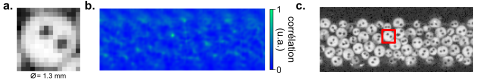
\includegraphics[scale=1]{../Figures_chap_exp/correlation_grains_1.pdf}
\caption[Détection des grains par PTV]{\textbf{a.}\,Motif extrait de la première image d'une acquisition. \textbf{b.}\,Image de corrélation du motif de gauche avec la dernière image de l'acquisition. \textbf{c.}\,Position détectée du motif de gauche dans la dernière image de l'acquisition. La position détectée correspond au maximum de corrélation, représenté par la tâche blanche la plus claire, au centre de l'image de corrélation.}
\label{fig:correl}
\end{figure}



\begin{figure}[p]
\centering	
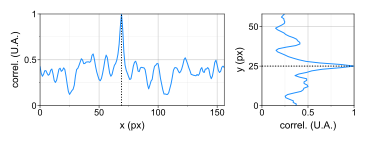
\includegraphics[scale=1]{../Figures_chap_exp/correlation_grains_2.pdf}
\caption[Profil de corrélation]{Coupes transversales horizontale et verticale de la matrice de corrélation de la Figure\,\ref{fig:correl}, centrées sur le maximum de corrélation. Les deux coupes montrent que le maximum est situé au sommet d'un halo, qui peut être ajusté par une fonction gaussienne.}
\label{fig:gausscor}
\end{figure}


\begin{figure}[p]
\centering	
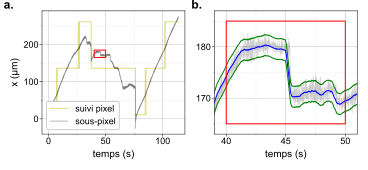
\includegraphics[scale=1]{../Figures_chap_exp/tracking_grains.pdf}
\caption[Suivi du mouvement d'un grain]{\textbf{a.}\,Suivi du mouvement d'un cylindre au cours d'une expérience. Un millimètre est balayé par 8 pixels. Nous observons la discrétisation et les oscillations rapides de la position au pixel (ligne jaune), et la position sous-pixel (ligne grise). L'intérieur du rectangle rouge est reproduit à droite. \textbf{b.}\,Détail du suivi du même cylindre. La courbe grise représente le suivi sous-pixel, et la courbe bleue représente la moyenne glissante sur 40 images de la position mesurée. La largeur du bruit associé au suivi, de l'ordre de \SI{2}{\micro\meter}, est déterminée par l'écart type médian des positions des cylindres lorsqu'ils sont immobiles, et est représentée par les deux courbes vertes.}
\label{fig:trackingres}
\end{figure}







\subsubsection{Amélioration de la résolution par PTV}



Afin d'améliorer la résolution du suivi des cylindres et de la placer en dessous de l'échelle du pixel, nous avons implémenté une méthode de \textit{Particle Tracking Velocimetry} (PTV). Il s'agit d'une interprétation lagrangienne de la \textit{Particle Image Velocimetry} (PIV)\,\cite{raffel_particle_2007}, reposant sur les mêmes principes généraux.

Cette méthode consiste en l'ajustement du pic de corrélation par une fonction gaussienne, au moyen d'un estimateur à trois points\,\cite{raffel_particle_2007}. En effet dans nos images, en raison de la largeur et de la forme circulaire des faces des cylindres, le maximum de corrélation est au centre d'un halo de hautes corrélations suffisamment symétrique pour être considéré Gaussien à l'ordre\,2 en son sommet (Fig.\,\ref{fig:gausscor}). Cet ajustement est effectué sur la matrice de corrélation normalisée et tronquée aux 4 points adjacents à sa valeur maximale. Ainsi si nous notons $\vec{\Delta} = \left[\Delta_x,\Delta_y\right]$ la position du maximum de la matrice de corrélation $r$, et donc la position du motif au pixel, nous pouvons définir $\vec{\delta}=\left[\delta_x,\delta_y\right]$ l'écart sous-pixel donné par l'ajustement :

\begin{align}[left=\empheqlbrace]
\begin{split}
\delta x &=\frac{1}{2}\times \dfrac{\ln(r_{i-1,j})-\ln(r_{i+1,j})}{\ln(r_{i-1,j})-2\times\ln(r_{i,j})+\ln(r_{i+1,j})}\\
\delta y &=\frac{1}{2}\times \dfrac{\ln(r_{i,j-1})-\ln(r_{i,j+1})}{\ln(r_{i,j-1})-2\times\ln(r_{i,j})+\ln(r_{i,j+1})}
\end{split}
\end{align}

La valeur de la position sous-pixel du centre du halo, et donc du motif, est alors $\vec{D} = \vec{\Delta}+\vec{\delta}$.

\subsubsection{Évaluation de la résolution par PTV}



\begin{figure}[hbt]
\centering
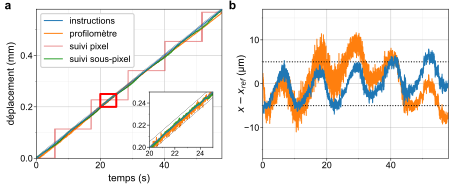
\includegraphics[scale=1]{../Figures_chap_exp/figure_S2_res_only.pdf}
\caption[Évaluation de la résolution de la PTV]{Évaluation de la résolution du suivi sous-pixel. \textbf{a.}\,Le déplacement commandé $x_{com}$ est une rampe de position à vitesse fixée (courbe bleue), mesurée par un profilomètre confocal $x_{prof}$ (orange). La mesure pixel (rose) est discrétisée, et la mesure  sous-pixel $x_{opt}$ (verte) est comprise dans une gaine de \SI{+-5}{\micro\meter} autour de la valeur de commande. \textbf{b.}\,Écart entre la position mesurée par le suivi sous-pixel $x_{opt}$ et la position de commande $x_{com}$ (bleu), ainsi qu'entre $x_{opt}$ et $x_{prof}$ (orange). La périodicité observée correspond aux changements de valeur du suivi au pixel.}
\label{fig:trackingres2}
\end{figure}


Afin d'évaluer la précision de cette méthode nous l'avons testée sur des grains en déplacement contrôlé. Nous avons créé plusieurs scripts de déplacement permettant de contrôler
%\href{https://youtu.be/???}{\textcolor{black}{informatiquement}}
informatiquement
la position de la platine motorisée et donc des blocs et cylindres qui en sont solidaires. Pour déterminer la résolution de la méthode de suivi, une translation à vitesse constante de \SI{10}{\micro\meter\per\second} est imposée au bloc inférieur, sans chargement normal. Afin de s'assurer de la bonne exécution des commandes par la platine, nous mesurons sa position à l'aide d'un profilomètre confocal commercial, d'une résolution de l'ordre d'un micromètre. Nous comparons ensuite la valeur de commande $x_{com}(t)$, la mesure du profilomètre $x_{prof}(t)$, et la mesure du suivi des grains solidaires du bloc en translation $x_{opt}(t)$ (Fig.\,\ref{fig:trackingres2}a). Les trois courbes suivent la même tendance, et la déviation standard de $x_{com}(t)-x_{opt}(t)$ vaut \SI{1.5}{\micro\meter}. Nous quantifions la précision du suivi à l'aide de la règle des 3 sigmas (incluant 99.7\% des valeurs), ce qui donne une limite de résolution de \SI{5}{\micro\meter}.

Une observation plus fine de l'écart entre la commande et le suivi optique révèle que $x_{com}(t)-x_{opt}(t)$ oscille de manière périodique (Fig.\,\ref{fig:trackingres2}b, courbe bleue). Cette même oscillation apparaît également lorsque l'on calcule $x_{com}-x_{prof}$ (courbe orange), et ne peut donc pas être imputée au mouvement de la platine, mais bien au suivi des cylindres. La limite de résolution déterminée précédemment de l'ordre de \SI{5}{\micro\meter} n'est donc en réalité pas due à une erreur aléatoire mais à un biais périodique. Les oscillations correspondent aux changements de valeur du suivi au pixel, et représentent un défaut majeur de notre méthode de suivi. Elles sont le facteur limitant dans les mesures de déplacements supérieurs ou de l'ordre d'un pixel, soit \SI{120}{\micro\meter}. En revanche, lorsque le déplacement mesuré est beaucoup plus faible que la taille d'un pixel, l'amplitude du bruit associé à la mesure optique est de l'ordre d'un micromètre.


\subsection{Traitement des données de suivi optique}


Les données brutes nous renseignent sur les mouvements absolus des cylindres au cours du temps. Nous effectuons plusieurs traitements sur celles-ci afin d'en faciliter l'analyse.

Le repère utilisé dans cette section est celui de l'interface, c'est à dire que l'axe horizontal $\vec{e_x}$ coïncide avec l'interface, et l'axe vertical $\vec{e_y}$ lui est perpendiculaire, orienté vers le haut. Les cylindres sont indexés par un entier $i$, et leurs positions sont notées $\vec{X}_i = (x_i,\,y_i)$.



\subsubsection{Classement des grains}
\label{sec:classement}



Afin de raffiner l'analyse des mouvements des cylindres, ceux-ci doivent être catégorisés en fonction de leur position sur le bloc relativement à l'axe de l'interface. Les différentes catégories sont les suivantes :

\begin{itemize}
\bitem $\{boundary\}$ et $\{bulk\}$ : Les cylindres solidaires d'un bloc solide sont catégorisés dans $\{boundary\}$, tandis que les cylindres libres sont dans la catégorie $\{bulk\}$. Chaque cylindre se voit attribuer manuellement une des deux catégories au moment de leur détection initiale. Les cylindres de la catégorie $\{boundary\}$, en les considérant bien répartis de part et d'autre de l'interface, permettent de définir $\bar{y} = \left\langle y_i\right\rangle_{i\in\{boundary\}}$ la hauteur approximative de la ligne d'interface, et $\bar{x}= \left\langle x_i\right\rangle_{i\in\{boundary\}}$ la position horizontale du centre des blocs.
\end{itemize}

Les catégories suivantes ne sont définies que pour les cylindres catégorisés dans $\{boundary\}$.

\begin{itemize}
\bitem $\{top\}$ et $\{bottom\}$ : les cylindres tels que $y_i>\bar{y}$ sont dans $\{top\}$, les autres $\{bottom\}$.

\bitem $\{left\}$, $\{middle\}$ et $\{right\}$ : Ces catégories ne sont pertinentes que dans le cas de l'interface avec œil granulaire. Les cylindres tels que $\abs{x_i-\bar{x}}<\ell_{eye}/2$ (appartenant à l'œil granulaire) sont catégorisés dans $\{middle\}$. Parmi les autres, ceux tels que $x_i<\bar{x}$ sont dans $\{left\}$, et tels que $x_i>\bar{x}$ dans $\{right\}$. Nous définissons également $\{solid\}=\{left\}\cup\{right\}$ et $\{eye\}=\{middle\}$.

\bitem Classification par paires : Les cylindres de $\{boundary\}$ étant généralement disposés de manière symétrique de part et d'autre de l'interface, il est possible de les classer par paire à partir de leur position initiale, soit manuellement, soit automatiquement. Pour qu'une paire de cylindres $(i,j)$ soit valide, il faut tout d'abord que l'un soit dans $\{top\}$ (sans perte de généralité $i$), l'autre dans $\{bottom\}$, et tous les deux dans la même portion d'interface dans le cas du système à œil granulaire. Le critère d'appariement est alors
\nopagebreak[4]
\begin{align}[left=\empheqlbrace]
\begin{split}
\forall m  \in\{bottom\},&\quad\abs{x_i-x_j}<\abs{x_i-x_m}\\
\forall n  \in\{top\},&\quad\abs{x_i-x_j}<\abs{x_n-x_j}
\end{split}
\end{align}

\end{itemize}

%Dans les définitions des sections suivantes, nous considèrerons uniquement les grains de la catégorie $\{boundary\}$, c'est à dire les grains solidaires des blocs solides.




\subsubsection{Correction du suivi des grains}
\label{sec:rotat}

\begin{figure}[htb]
\centering
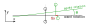
\includegraphics[scale=1]{../Figures_chap_exp/figure_5_rotat.pdf}
\caption[Correction de la rotation de l'interface]{Effet de la rotation de l'interface relativement à la caméra sur le déplacement mesuré des grains. Cet effet est corrigé en temps réel par un ajustement de la position de l'interface.}
\label{fig:rotat}
\end{figure}

La mesure de l'évolution de la position d'un cylindre et du glissement interfacial peuvent être perturbées par des mouvements parasites. Les principaux sont la rotation et la translation des blocs dans leur ensemble lors de leur cisaillement dues à la flexibilité du cadre de la presse, et les déformations élastiques des blocs.


\myparagraph{Influence de la rotation de l'interface}

La rotation et le déplacement de l'axe de l'interface augmentent avec la force cisaillante appliquée au système. Leur amplitude peut atteindre 1 mm et \ang{0.2}, ce qui peut mener à détecter à tort un glissement relatif entre deux cylindres de part et d'autre de l'interface (Fig.\,\ref{fig:rotat}). De plus le réglage de l'horizontalité de la caméra a une précision de seulement \ang{0.1}. Il n'est donc pas raisonnable de considérer que les axes de la caméra coïncident à tout moment avec l'axe naturel de l'interface.

Afin d'éliminer les déplacements parasites, nous projetons les coordonnés mesurées dans le référentiel de la caméra sur le référentiel naturel de l'interface. Pour ce faire, nous mesurons la position et la rotation de l'interface par rapport à l'axe horizontal de la caméra $\vec{e}_{x,cam}$. La classification des cylindres dans les catégories $\{top\}$ et $\{bottom\}$ permet de définir deux ajustements linéaires respectivement de la position des cylindres solidaires du bloc supérieur $y_{top}(t)=a_{top}(t)\times x_{cam}+b_{sup}(t)$, et du bloc inférieur $y_{bot}(t)=a_{bot}(t)\times x_{cam}+b_{bot} (t)$. Ces deux ajustements permettent à leur tour de définir l'équation de la position $y_{int}$ de l'interface dans le référentiel de la caméra $y_{int} = (y_{bot}+y_{top}) = a(t) \times x_{cam} + b(t)$. Pour un point de coordonnées $(x_0,y_0)$ dans le référentiel de la caméra, ses nouvelles coordonnées $(x_1,y_1)$ dans le référentiel de l'interface sont


\begin{align}[left=\empheqlbrace]
\begin{split}
x_1&= \dfrac{x_0+ay_0-a b}{\sqrt{a^2+1}} \\
y_1&= \dfrac{y_0-a x_0-b}{\sqrt{a^2+1}}
\end{split}
\end{align}

Cette projection dans le référentiel naturel de l'interface est effectuée lors du traitement des données issues du suivi des cylindres, et précède tous les autres traitements et calculs appliqués au cours de l'analyse.

\myparagraph{Influence de la différence de hauteur des cylindres}


\begin{figure}[htb]
\centering
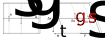
\includegraphics[scale=1]{../Figures_chap_exp/figure_S1.pdf}
\caption[Effet de la déformation des blocs]{Effet de la déformation des blocs sur le déplacement mesuré des grains. Cet effet est négligeable dans le cadre de notre étude.}
\label{fig:defor}
\end{figure}

La différence de hauteur $h$ entre les paires de faces de cylindres de l'œil granulaire et celles des portions solides est de l'ordre de \SI{4}{\milli\meter}, et peut introduire des erreurs dans la mesure des déplacements en raison de la déformation des blocs en cisaillement (Fig.\,\ref{fig:defor}). Évaluons l'amplitude de cet effet dans le cas le plus défavorable. Nous considérons que la force de cisaillement atteint $F_S=\SI{1500}{\newton}$, avec $A=150\times\SI{10}{\milli\meter\squared}$ l'aire de contact entre les deux blocs, alors $\sigma_{xy}=F_S/A=10^6\,\text{Pa}$. Le déplacement $\delta x$ entre deux faces d'une même paire, à distance $h$, est alors

\begin{equation}
\delta x = \frac{2h\sigma_{xy}}{E/(2(1+\nu))}
\end{equation}

Ainsi nous trouvons $\delta x_g=\SI{9}{\micro\meter}$ et $\delta x_s=\SI{5}{\micro\meter}$. L'écart entre les deux quantités est inférieur à la résolution obtenue par le suivi PTV, et l'effet réel peut donc être négligé.






\subsubsection{Format des données}
\label{sec:optiquesdonnées}

Les données brutes acquises par la caméra sont des images en nuances de gris sur 12 bits, cependant le format utilisé pour le traitement des images est limité à 8 bits. Les images sont sauvegardées sans compression ni traitement sous le format \texttt{tiff}. Les mesures détaillées dans cette section et la suivante sont effectuées sous MatLab\,\cite{matlab_9501067069_2018}, et les données sont sauvegardées sous le type \texttt{double}, permettant une précision de l'ordre de 16 chiffres significatifs. Les données ainsi obtenues sont manuellement traitées pour éliminer les erreurs potentielles (fausses détections, cylindres mal suivis, images corrompues). Une partie des données est exportée après traitements sous Python3, pour être analysée avec les données d'acquisition électronique (Sec.\,\ref{sec:electroniquedonnées}).







\subsection{Expérience simulée et conditions réelles}
\label{sec:obsoptique}


\begin{figure}[htb]
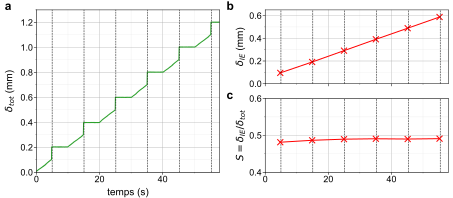
\includegraphics[scale=1]{../Figures_chap_exp/figure_S2_delta_only.pdf}
\caption[Définition de $\delta_{IE}$ et $S$]{Déplacement d'un seul des blocs commandé par un script. \textbf{a.}\,Mesure du déplacement interfacial $\delta_{tot}$. Les évènements détectés sont marqués par les lignes en pointillés noirs. \textbf{b.}\,Évolution du glissement inter-évènement $\delta_{IE}$. \textbf{c.}\,Évolution du glissement inter-évènement normalisé $S$.}
\label{fig:delta}
\end{figure}


Dans cette section nous présentons brièvement le comportement typique dit de \textit{stick-slip} que nous observons dans les expériences que nous avons menées, et détaillons les définitions des grandeurs d'intérêt que nous étudions, par le biais de l'exemple d'une expérience simulée.

\subsubsection{Mouvement de stick-slip et glissement inter-évènement}
Lors d'une expérience de cisaillement de deux blocs pressés, le mouvement relatif des blocs est saccadé. Dans un modèle idéal, ce mouvement est constitué d'une alternance de phases de \textit{stick} de durée $T$, durant lesquelles le déplacement relatif des blocs à l'interface est nul, et d'évènements rapides de \textit{slip}, où l'interface glisse d'une distance $d_0$. Cette succession de phases est périodique, de période $T$ dépendant des paramètres de chargement. Le déplacement relatif de l'interface $\delta_{tot}^{ideal}(t)$ est alors une fonction constante par morceaux

\begin{equation}
\delta_{tot}^{ideal}(t)= d_0\times\floor{\frac{t}{T}}
\end{equation}

Dans une expérience réelle de stick-slip, le mouvement comporte une alternance de longues phases de stick (de durée moyenne $\mean{T}$, de l'échelle de la seconde), durant lesquelles le déplacement relatif des blocs est quasi-nul (à l'échelle du micromètre), et des évènements courts de slip (à l'échelle de la centaine de milliseconde), qui concentrent la majeure partie du déplacement (à l'échelle du millimètre). Dans certaines configurations que nous étudions le glissement ayant lieu entre les phases de slip peut atteindre le même ordre de grandeur que celui ayant lieu pendant celles-ci. Nous vérifions à l'aide d'une expérience simulée que le suivi des grains que nous avons implémenté permet bien de mesurer le glissement entre les évènements de slip.


\subsubsection{Expérience simulée : stick-slip avec glissement inter-évènement}



Afin de simuler un mouvement de stick-slip comportant du déplacement lent entre les évènements de slip, nous contrôlons la position du bloc inférieur non-chargé, au moyen de la platine motorisée, pilotée par un script (Fig.\ref{fig:delta}a). Les cylindres solidaires du bloc sont suivis par imagerie. Les instructions données sont des cycles de 5 secondes sans mouvement, 5 secondes de déplacement uniforme à \SI{20}{\micro\meter\per\second} (glissement lent), et un saut brusque de \SI{100}{\micro\meter} (évènement de slip).


Cette expérience a pour but de vérifier que notre méthode de suivi et de traitement mesure bien \SI{100}{\micro\meter} de déplacement par phase de slip, et \SI{100}{\micro\meter} par phase inter-évènement. Pour ce faire nous mesurons le déplacement $\delta_{tot}$, détectons les instants $\{t_{k}\}_{k\in\mathbb{N}}$ des évènements de slip, et en déduisons le déplacement inter-évènement $\delta_{IE}$. Les mesures de ces quantités dans l’expérience simulée et leurs définitions dans les expériences réelles sont détaillées dans les trois sections suivantes.




\subsubsection{Glissement interfacial total}
\label{sec:totslip}

Pour l'expérience simulée, afin de déterminer le déplacement total des cylindres $\delta_{tot}$, nous effectuons la moyenne des déplacements de tous les grains. Nous vérifions bien que ce suivi est correct (Fig.\,\ref{fig:delta}a).


Dans le cas d'une expérience réelle, l'application d'une force entraîne un déplacement général de tous les grains dans le sens du cisaillement, $\delta_{tot}$ est alors défini comme déplacement \textit{relatif} des blocs à l'interface. Cette mesure est permise par le classement des grains selon leur appartenance à la catégorie $\{top\}$ ou $\{bottom\}$, donnant

\begin{equation}
\delta_{tot}(t) = \mean{x_i}_{i\in\{top\}}(t) - \mean{x_j}_{j\in\{bottom\}}(t)
\end{equation}


Pour d'autres usages, il est possible de raffiner cette quantité par portion d'interface ou par paire de grains. Par exemple le déplacement relatif des  cylindres dans la partie solide-solide de l'interface avec œil granulaire est noté $\delta_{tot}^{solid}(t)$, et est défini comme

\begin{equation}
\delta_{tot}^{solid}(t) = \mean{x_i}_{i\in\{top\}\cap\{solid\}}(t) - \mean{x_j}_{j\in\{bottom\}\cap\{solid\}}(t)
\end{equation}

Nous cherchons maintenant à distinguer le mouvement effectué durant les phases de slip du glissement lent effectué entre celles-ci.


\subsubsection{Détection des évènements de glissement rapides}
\label{sec:detecoptique}

Afin d'étudier indépendamment chaque phase du mouvement, il nous faut détecter les évènements de glissement rapide. Cette détection est effectuée par un filtrage passe-haut de $\delta_{tot}(t)$ mettant en évidence ses changements brusques. Nous obtenons ainsi une liste de temps $\{t_{k}\}_{k\in\mathbb{N}}$ correspondant à chaque évènement de glissement rapide (Fig.\,\ref{fig:delta}, lignes pointillées). Ces temps permettent également de synchroniser les mesures optiques avec les mesures électroniques, dans lesquelles les évènements sont repérés par un signal accélérométrique (Sec.\,\ref{sec:accel}).

Afin de définir les limites des phases de stick, il nous faut considérer une marge autour de chaque temps $t_k$ assurant qu'aucun mouvement d'une phase de slip ne soit comptabilisé dans une phase de stick. Nous notons $t_k^-$ et $t_k^+$ les temps limites de chaque évènement, $t_k^- = t_k-\tau^-$ correspondant à l'instant juste avant l'évènement de glissement, et $t_k^+ = t_k+\tau^+$ au temps à partir duquel l'interface est stabilisée. La valeur de $\tau^-=\SI{0.05}{\second}$ est choisie constante, tandis que la valeur de $\tau^+$ est définie en fonction du comportement de l'interface. Elle est prise de façon à s'assurer que la phase de glissement rapide soit bien terminée, et que les vibrations de la table optique supportant la presse, dues à l'évènement, soient atténuées. La durée de cette phase de vibrations dépend de la quantité d'énergie relâchée par l'évènement, elle-même proportionnelle à la période à laquelle les phases de slip se répètent. Ainsi nous définissons $\tau^+$ comme une fonction croissante de $\mean{T}$, variant de \SI{0.15}{\second} à \SI{0.5}{\second}. Dans l'expérience de stick-slip simulée, les évènements sont bien détectés (Fig.\ref{fig:delta}a, lignes pointillées).


\subsubsection{Glissement inter-évènement}

La détection des évènements de glissement rapide permet enfin de définir le glissement inter-évènement $\delta_{IE}(t)$. Il correspond au glissement interfacial entre les évènements de glissement rapide, cumulé tout au long de l'expérience, et est défini comme

\begin{equation}
\delta_{IE}(t) = \delta_{tot}(t)-\sum_{t_k\leq t}\Big(\: \delta_{tot}(t_k^+)-\delta_{tot}(t_k^-)\:\Big)
\end{equation}

Cette grandeur peut se calculer pour une catégorie des cylindres suivis, et est alors notée avec la catégorie en question en exposant, $\delta_{IE}^{eye}$ pour la catégorie $\{eye\}$ par exemple. Lorsque nous représentons $\delta_{IE}(t)$, nous indiquons uniquement ses valeurs aux différents $t_k^+$ (Fig.\,\ref{fig:delta}), c'est à dire

\begin{equation}
\delta_{IE}(t_k^+) = \delta_{tot}(t_k^+)-\sum_{\kappa\leq k} \Big(\:\delta_{tot}(t_\kappa^+)-\delta_{tot}(t_\kappa^-)\:\Big)
\end{equation}


Dans le cas de l'expérience simulée présentée, la valeur de $\delta_{IE}(t)$ imposée par le script augmente de \SI{100}{\micro\meter} entre chaque évènement. La valeur que nous mesurons en pratique montre bien cette augmentation (Fig.\,\ref{fig:delta}b), bien que la valeur mesurée soit 1 à 2\% plus faible, en raison de la marge $\tau^-+\tau^+$ prise autour de chaque $t_k$.

\pagebreak

L'extraction du glissement inter-évènement et sa représentation sous la forme de la suite de ses valeurs permettent de déterminer la proportion du déplacement total de l'interface se faisant entre les évènements de glissement rapide. Afin d'évaluer cette proportion, nous définissons le glissement inter-évènement normalisé $S(t)$ comme

\begin{equation}
S(t) = \dfrac{\delta_{IE}(t)}{\delta_{tot}(t)}
\end{equation}

De même que $\delta_{IE}$ nous représentons généralement cette quantité de manière discrète, à chaque $t_k^+$ (Fig.\,\ref{fig:delta}c). Cette mesure de la proportion de glissement effectuée entre les évènements de glissement rapide est sous-estimée en raison de la largeur de la marge $\tau^-+\tau^+$ prise autour de chaque $t_k$. Dans le cas de l'expérience simulée, nous trouvons $S\sim 0.49$, pour une valeur attendue de $S=0.5$, l'écart s’expliquant par cette largeur.




\section{Conclusion}

Au cours de ce chapitre nous avons présenté le dispositif expérimental que nous avons développé durant cette thèse. Ce dispositif nous permet de presser et cisailler des plaques minces de PMMA, de plusieurs géométries et pouvant encapsuler un milieu granulaire bidimensionnel, en ayant une mesure précise des forces que nous leur appliquons. Les plaques sont équipées d'une électronique de précision permettant l'acquisition simultanée du signal de 20 rosettes (60 jauges) à une fréquence de \SI{4}{\mega\hertz}, nous offrant la résolution et la rapidité nécessaires à la mesure du champ des déformations à l'interface qu'elles forment lors d'une expérience. Cette mesure est complétée par un suivi par imagerie de la position des grains à l'interface qui nous permet de caractériser en détail les déplacements de ceux-ci à l'échelle micrométrique. Nous avons également introduit des quantités d'intérêt pour l'étude de l'interface en œil granulaire présentée dans le Chapitre\,\ref{sec:chaparticle}, notamment les mesures de glissement interfacial durant et entre les évènements de glissement rapide.

Grâce à ce dispositif et à la précision de son instrumentation, nous étudions et présentons par la suite les interfaces granulaires, et notamment l'influence d'une hétérogénéité, sous la forme d'un œil granulaire, sur le comportement de celles-ci.





